% Chapter 1
\chapter{Introduction} % Main chapter title

\label{chap:introduction}

%----------------------------------------------------------------------------------------


\section{Star formation in clustered environments}

\subsection{Molecular Clouds}

Molecular clouds are the dense regions of the interstellar medium (ISM) where stars are forming. They contain about half the mass of the ISM in $<2$\% of its volume \citep{Ferriere:2001gv}. High densities ($n > \SI{100}{\centi\meter\raiseto{-3}}$) of mostly molecular hydrogen and low temperatures ($< \SI{20}{\kelvin}$) distinguish molecular clouds (sometimes called \textit{dark clouds}) from the various other components of the ISM in galaxies: the Warm Neutral Medium (WNM), the Warm Ionized Medium (WIM), and the other cold phase of the ISM, the Cold Neutral Medium (CNM), which is thought to be the parent region in which molecular clouds are formed \citep{Kennicutt:2012ey}. In addition to molecular hydrogen, molecular clouds also contain Helium (10\% by number), dust ($\sim 1\%$ by mass), CO ($\sim \num{1e-4}$ by number), and traces of many other molecules.

Observations of molecular clouds reveal that they are highly structured with often a filamentary pattern [cite shaye?]. While the literature proposes multiple classifications for the various structures found in molecular clouds, we chose to focus only on two structures which are key to this work: clusters, which are more local associations of stars in virial equilibrium \citep{Lada:2003il}; and dense cores, which are sites where stars form individually or in systems of small multiples \citep{Williams:2000wl}. Clusters are formed of multiple cores, but cores can also be found outside of clusters, in the field. In the classical picture, clouds are thought to fragment into clusters, which still contain many times the Jean's mass - the minimum mass for gravitationally-bound cores \citep{Larson:1994cj} which are also called prestellar cores \citep{DiFrancesco:2007vg}.

%[The structure of clusters itself is of great interest to study the mechanisms at stake in star formation, because it gives information about the cluster's origins \citep{Lada:2003il}. Clusters are believed to be relatively short-lived, because the stars it forms can disrupt its gravitational equilibrium. Typical timescales for clusters are on the order of \SI{100}{\mega\year} \citep{Lada:2003il}. ]

Approximately 60\% of all stars are thought to form in embedded, young stellar clusters of 1-\SI{3}{\mega\year} with 100 or more stars \citep{Porras:2003kxa,Allen:2007wqa}. These $>$100 star clusters have characteristic sizes of 2-4 parsecs (pc) with peak surface densities of 100-\si{1000} stars per square parsec and a typical median distance between nearest neighbor young stellar objects (YSOs) of 0.03 to 0.06 pc \citep{Gutermuth:2009gca}.

Because star-forming clusters are surrounded by interstellar matter from the parent molecular cloud, they usually cannot be studied at optical wavelengths, due to the large obscuration from dust grains along the line of sight. Infrared observations can be used to probe these structures since the dust can acquire sufficient temperature to emit thermally from the mid-infrared to millimeter and radio wavelengths. 

The high density of YSOs within clusters, combined with their typical distances of few hundredths of parsecs requires a high angular resolution in order to capture the relevant spatial scales at which accretion mechanisms are happening throughout the YSO's life. [Millimeter-wave and radio observations can provide ..., but]



[Molecular hydrogen is believed to form by recombination on the surface of dust grains [hollenbach and salpeter 1971, and are only able to survive from UV photodissociation within these obscured clouds.]

\subsection{Star formation}

\subsubsection{Standard models}

A considerable amount of literature exists on star formation and the various physical processes involved in forming stars. In this section, we review some of the most standard views that describe how stars are born and grow to acquire their final masses.

\paragraph{Gravitational collapse}

A simple way to derive characteristic quantities related to the formation of stars is to consider a pre-stellar core as a clump of spherical, uniform, isothermal gas in hydrostatic equilibrium. For such a system, the Virial theorem applies, which describes the balance between the gravitational potential of the clump and the kinetic thermal energy within the gas. In other words, in hydrostatic equilibrium, the core's self-gravity is compensated by the internal pressure caused by the temperature of the gas which prevents the collapse of the core. For the same radius and temperature, a core with more mass will lead to a runaway collapse until another force eventually compensates gravity - in our case, this force corresponds to the radiation pressure that is created when nuclear fusion is ignited and the star is born. While simplistic, this treatment leads to a straightforward derivation of critical timescales, sizes, and masses that form a good starting point for more elaborate theories. 

First, it is important to determine what are the characteristic timescales of star formation. In the core with a uniform density, the simplest timescale to define is called the free-fall time: this is the time it takes for the total gravitational collapse of a spherically-symmetric clump of uniform density $\rho$ if only the force of gravity is considered\footnote{Note that the scaling coefficient associated with the free-fall time can change among authors; these are merely scaling relations and do not pretend to be exact}, 
\begin{equation}
\tff \sim \left(\frac{3\pi}{32 G\rho}\right)^{-1/2}\sim \SI{2.1}{\mega\year}\left(\frac{\rho}{\SI{e-21}{\gram\per\raiseto{3}\centi\meter}}\right)^{-1/2}.
\end{equation}
The free-fall time is usually a lower limit on the collapse timescale, since there will always be some thermal pressure that will resist gravity and slow down the infall of gas into the potential well. 

The other relevant quantity that involves time is the sound speed in the cloud, $\cs = (kT/(\mu m_H))^{1/2}$, where $\mu$ is the mean molecular weight of the gas and $m_H$ the mass of hydrogen. For a given spatial scale $R$, the sound-crossing time is defined as $\ts = R/\cs = \SI{4.9e5}{\year}\left(\frac{R}{\SI{0.1}{\pc}}\right)\left(\frac{\cs}{\SI{0.2}{\kilo\meter\per\second}}\right)^{-1}$. This is the time it takes for a wave to cross the scale $R$ while traveling at the sound speed. 

Intuitively, if $\tff<\ts$, the core of size $R$ will start its gravitational collapse, while it will remain stable otherwise. This corresponds to a characteristic sizescale that is called the Jeans length, and corresponds to the characteristic sizescale of gravitational instability within a cloud \citep{McKee:2007bd}:
\begin{equation}
 \lambdaJ = \cs\times\tff = \SI{0.43}{\pc}\left(\frac{\cs}{\SI{0.2}{\kilo\meter\per\second}}\right)\left(\frac{\rho}{\SI{e-21}{\gram\per\raiseto{3}\centi\meter}}\right)^{-1/2}.
 \end{equation} 

The Jeans mass is the amount of mass within a sphere of diameter \lambdaJ, and corresponds intuitively to the minimum mass a core needs to gather in order to trigger an gravitational collapse:
\begin{eqnarray}
\MJ &=& \frac{4\pi}{3}\rho\left(\frac{\lambdaJ}{2}\right)^3 \\
&=& \SI{0.61}{\Msun} \left(\frac{\cs}{\SI{0.2}{\kilo\meter\per\second}}\right)^3 \left(\frac{\rho}{\SI{e-21}{\gram\per\raiseto{3}\centi\meter}}\right)^{-1/2}
\end{eqnarray}

Note that this formalism completely ignores the material that surrounds the core while it collapses. In practice, the cloud exerts an external pressure on the core that needs to be taken into account when calculating the critical masses. This more elaborate case of a clump of self-gravitating gas on the verge of collapse that is immersed in a medium of external pressure $\Pext$ is called a Bonnor-Ebert sphere. It can be shown\citep{McKee:2007bd} that the sizescale is similar to the Jeans' length, and the mass scale is a few times smaller than the Jeans' mass, which stays well within the accuracy limits of our simple model.

Once the gas starts its gravitational collapse, nothing stops it until the central pressure and density reach values that trigger the ignition of nuclear fusion. This is the birth of the star. This new mechanism creates a large amount of radiation pressure that balances out the collapse and forms a new hydrostatic equilibrium. 

In practice, it is likely that a single core fragments into multiple centers of collapse, each of them exceeding the local Jeans mass. This would create systems of binaries or small multiples instead of single stars, a scenario that is currently favored [LARSON?].

As the core continues to collapse onto the star, more material falls inwards and the envelope adopts a density profile which decreases with increasing distance to the central object. Most models result in an infalling envelope with density profiles which follow laws from $r^{-1/2}$ to $r^{-2}$, an important observable that can be useful to test these theories. Some models of slowly-rotating infalling clouds suggest more complex density profiles for the envelopes \citep[e.g.][]{Ulrich:1976ho,Terebey:1984hi} than simple power laws, but are observationally difficult to constrain due to the small differences with traditional power-law envelopes and the small scales at which those differences occur (a few 100's of AU). Through conservation of angular momentum, some of the surrounding material naturally flattens into a centrifugally-supported flaring disk before it is fed to the star, and a cavity opens along the rotation axis of the system. The cavity opening can also be bolstered by mechanisms such as stellar winds and jets [REFERENCE].

The object now has three characteristic components: the star itself; the flattened disk; and a diffuse envelope with an open cavity, which constitutes a mass reservoir for future accretion onto the star.

Although most of the mass is contained in the $\textrm{H}_2$ gas, there is a small fraction of material in the form of dust grains of various sizes and populations. Despite their low mass, these grains play a very important role in determining the observable properties of YSOs, because of their tendency to absorb short wavelengths and radiate in the thermal infrared (see Section~\ref{subsec:dust}). 

%The accretion mechanism most commonly consists of Bondi accretion \citep{Bondi:1952fc}, and represents the transfer of mass from the envelope or the disk to the star. As the YSO moves through its parent cloud, it can also accrete more mass throughout its life that was not originally part of the original condensation that initiated the collapse. In these dense regions where multiple stars are forming, interactions between YSOs is more than likely and can significantly affect the final masses of stars.

%Various models exist for accretion, from a quasi-static slow process \citep{Shu:1977ef} to a very rapid and brutal process \citep[e.g.][]{Larson:1967ee}. \cite{McKee:2007bd} suggest that the infall process is most likely slowing down as a function of time, which complicates its observational validation. 


% , the speed of sound is $c_s = (kT/m)^{1/2}$.
%Perhaps the most elementary way to model the birth of a star consists of considering an isothermal sphere of self-gravitating gas (a core) on the verge of collapse, in hydrostatic equilibrium with its surrounding cloud medium of gas pressure \Pext. This is also called a Bonnor-Ebert sphere \citep{Ebert:1955wf,Bonnor:1956cy}, and the state of this sphere is said to be \textit{critically stable}, with a critical mass defined by $\Mcrit = 1.18\frac{c^4_s}{G^{3/2}}\Pext^{-1/2}$ \citep{Shu:1977ef}, where $c_s = (kT/m)^{1/2}$ is the speed of sound in the cloud. To put this in perspective using physical quantities, we have:
%\begin{equation}
%M_{BE} = 0.66 \left(\frac{T}{\SI{10}{\kelvin}}\right)^2 \left(\frac{\Pext/k_B}{\SI{3e-5}{\raiseto{-3}\centi\meter\kelvin}}\right)^{-1/2}\si{\Msun},
%\end{equation}
%where \Pext was normalized to mean kinetic pressure at the surface of molecular clouds \citep{McKee:2007bd}. The Bonnor-Ebert radius is $R_{BE} = 0.49 c_s/(G\rho_0)^{1/2}$,  which is comparable to the characteristic fragmentation size scale called the Jeans' length. Here $\rho_0$ is the uniform density of the core. 

%For a core of mass $M_{BE}$, the thermal pressure exactly compensates the gravitational forces. Collapse occurs for cores with mass $>M_{BE}$ when gravity overcomes the thermal pressure of the gas inside the sphere, which triggers the rapid mass growth of a central embryo towards infinitely high densities. In practice, the process stops when enough density is reached to ignite nuclear fusion and stabilize the embryo, which has just become a young stellar object. Even after the star is born, mass continues to fall into the potential well, emitting radiation and increasing the mass of the central object. Various scenarios exist for this phase of the accretion within individual cores, 




%Since the accretion rate can be linked to the observed luminosities as gas falls into the gravitational potential well, it is also an important outcome of a given collapse model.
%For low-mass star formation from cores that are marginally super-critical, the infall phase can be treated in the quasi-static limit \cite{Shu:1977ef} and follows this normalized form \citep[Eq.44,][]{McKee:2007bd}:
%\begin{equation}
%\dot{m}_{infall} = \num{1.54e-6} \left(\frac{T}{\SI{10}{\kelvin}}\right)^{3/2}\si{\Msun\per\year}.
%\end{equation}

%More massive stars follow an accretion behavior more similar to Bondi-Hoyle accretion
%Conserving its original angular momentum

%[Accretion rates are likely varying as a function of time {McKee:2007bd}, and can complicate the interpretation ]

%[Magnetic fields, turbulence, asymmetries and non-isothermal considerations all likely play role in this balance, but dramatically complicate the mathematical treatment of the problem. In order to introduce the basic concepts of star formation, these complex processes are ignored.]

%\citep{Myers:2014ct}; includes why accretion stops. Shu accretion for low mass, Bondi accretion at high mass?

\paragraph{YSO classification and characteristics}

We have determined that YSOs are composed of a star, a disk, and an envelope. The star is believed to be fairly well understood as a young object in hydrostatic equilibrium on its way to the main sequence. Depending on many parameters, the spatial distribution of gas in the disk and the envelope can be predicted by simple models, but in all likelihood is very complex, inhomogeneous, and asymmetric. 
%Often, the envelope is thought to open up a cavity around the poles of the rotating system, where material can escape the system (through outflows, for example [REFERENCE?]). 
For clarity, we will discuss here the simple models that can be used to describe the YSOs in the multiple stages of their evolution.

In the most common model of the evolution of young stars, there are four stages in the lifetime of a YSO. The first stage consists of a dense core right after the YSO is born. The disk is almost inexistent, the envelope still is dense and circularly symmetric. This is called Stage 0. As the gas falls onto the star, rotation of the entire system tends to clear out a cavity at both poles of the system. As the system evolves, the cavity opening angle grows, the density of the envelope decreases, and the size of the disk increases. When a YSO is Stage III, the envelope is almost entirely depleted.

The various stages of YSO (from 0 to III) have very distinct observational signatures, although are highly dependent on the viewing angle. The most commonly used tool to classify YSOs based on their SEDs is to use the spectral index, which corresponds to the mid-IR slope $\alpha$ in the log-log plots, with $\alpha = \textrm{d}(\lambda F_\lambda)/\textrm{d}\lambda$ between 2 to \SI{20}{\micro\meter} \citep{McKee:2007bd}.

\begin{enumerate}
\item Class 0: Most the of short-wavelength ($<\SI{10}{\micro\meter}$) light is highly obscured by the dust in the massive envelope. Most of the emission is around \SI{100}{\micro\meter} and into the submillimeter and radio regimes. If there is a disk, it is very small.
\item Class I: Light scatters at short wavelength off the dust grains to give us a hint at the embedded object, but it still very obscured. The envelope's mass is lower, and the disk extends to larger distances. The typical spectral index $\alpha$ is positive.
\item Class II: The YSO is now a pre-main sequence star, with a spectral index $-1.5 < \alpha < 0$ a significant circumstellar disk. This is traditionally referred to as a classical T-Tauri star.
\item Class III: Still a pre-main sequence star, but most of the accretion has stopped, and $\alpha < -1.5$. The envelope has almost completely disappeared.
\end{enumerate}

An illustration of canonical spectral energy distributions (SED) and density structure is shown in Fig/ [REF] for the four main stages, with parameters taken in \cite{Whitney:2003kc}. On the left of each picture, the SED is the measurable quantity when the YSO is unresolved at all wavelengths. The challenge is to estimate the density structure (to the right) by measuring the SED. The different lines plotted in the SEDs are different inclination angles, highlighting the enormous impact of the viewing angle on the potential interpretation of these SEDs. These models were run using the Hyperion software \citep{Robitaille:2011fc} with "OH5" dust \citep{Ossenkopf:1994tq}, as discussed in more details in Section~\ref{subsec:dust}.


\begin{figure}[!ht]
	\centering
	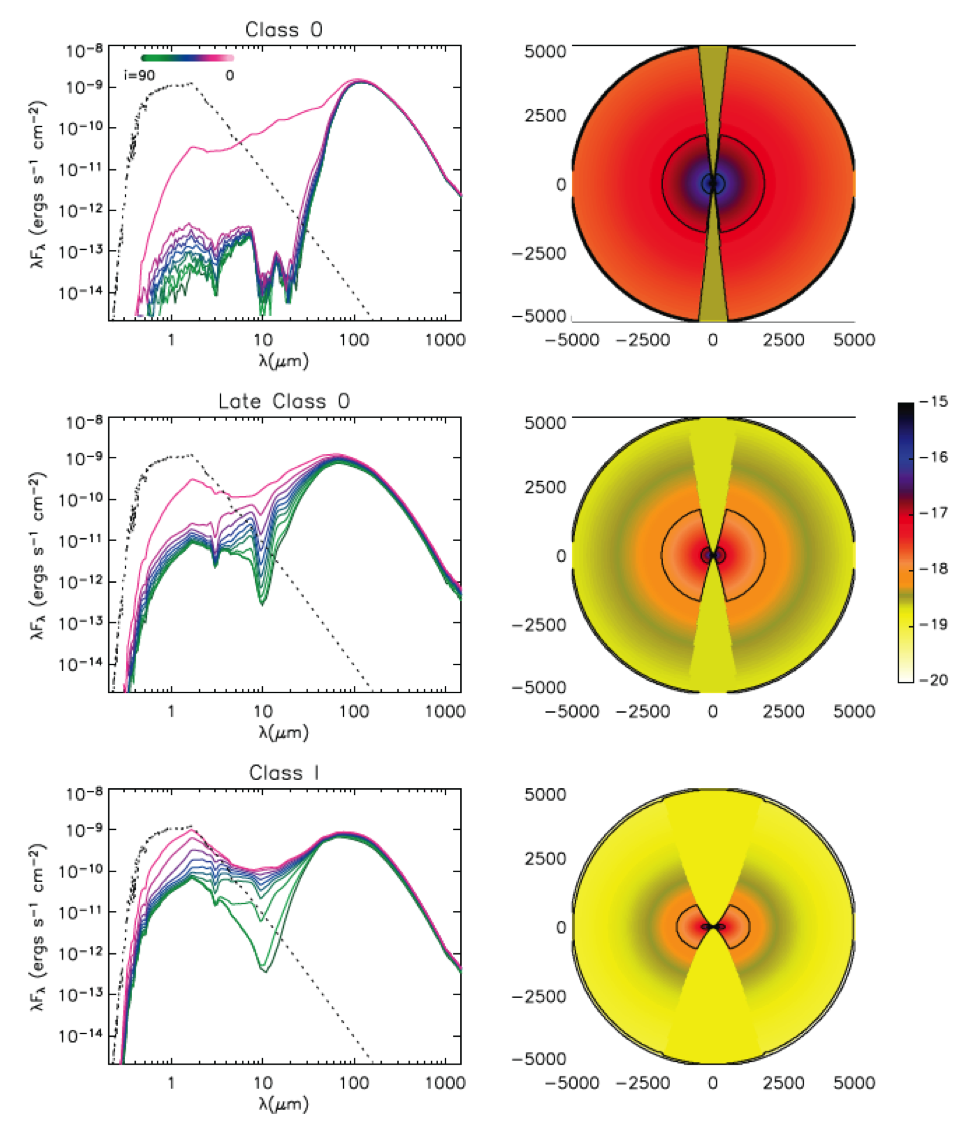
\includegraphics[width=\textwidth]{Figures/Whitney1.png}
	\caption[Stages 0 through I]{First stages of the birth of a star.}
	\label{fig:whitney1}
    \end{figure}
\begin{figure}[!ht]
	\centering
	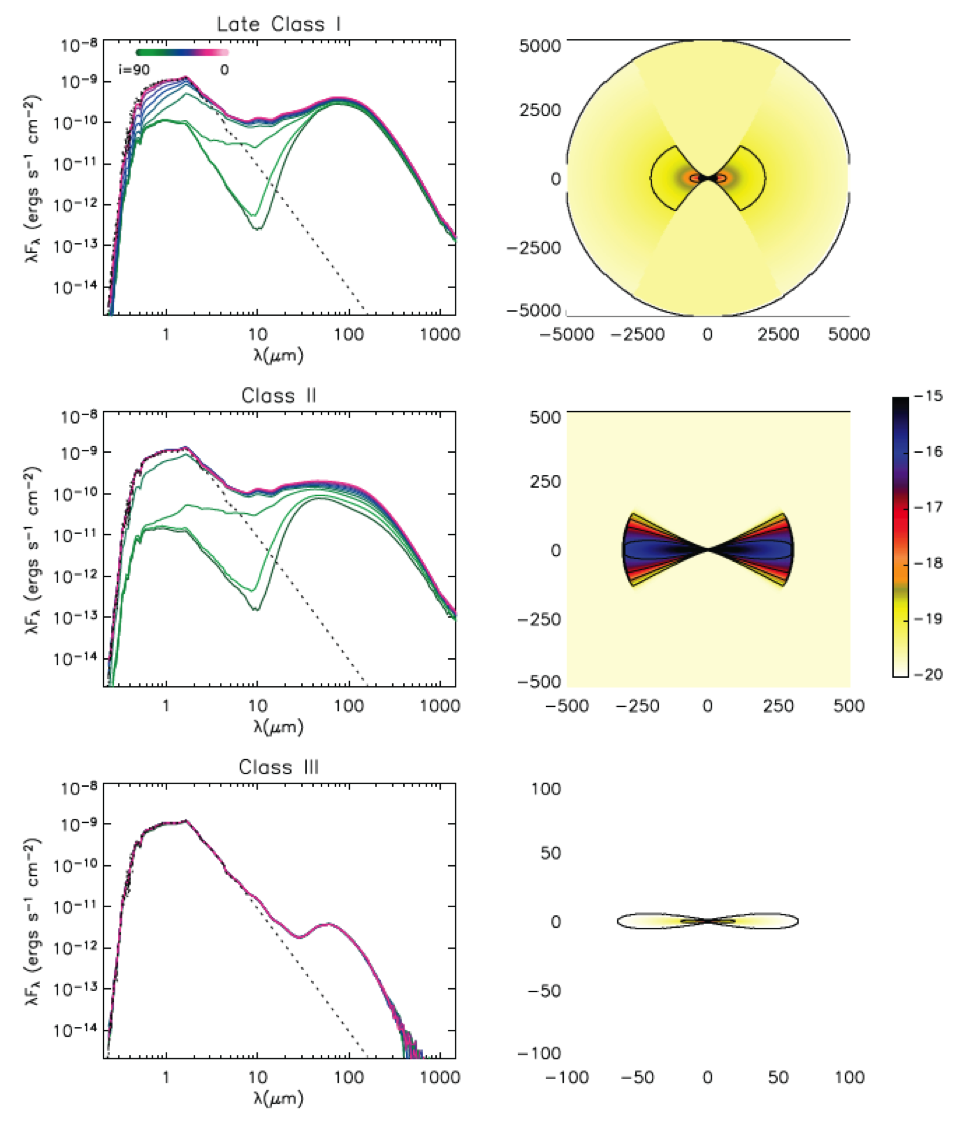
\includegraphics[width=\textwidth]{Figures/Whitney2.png}
	\caption[Stages I through III]{Last stages of the birth of a star, on its way to the main sequence.}
	\label{fig:whitney2}
    \end{figure}


\subsubsection{Mass accretion in clusters}


The discussion in the previous section represents a canonical view of how a single core collapses and forms a star. While it is convenient to assume that the core forms a fixed reservoir of gas that will determine the star's final mass, it is likely too simplistic, since these YSOs are preferentially forming inside of clusters close to multiple other YSOs and sharing a dense, often turbulent environment. 

The question of how stars acquire their final mass is a key problem in studying star formation. Does dense gas fragment into isolated centers of collapse? Do young stars competitively accrete material from a surrounding common reservoir? Do gravitational interactions between forming young objects play a significant role in setting the final stellar mass function? Better observational understanding of these clusters is necessary to address these questions and to discriminate between the different models, as noted by \cite{Bonnell:2006ee}, \cite{Offner:2011ex} and \cite{Myers:2011fy}.

Given the typical stellar separations in clusters with fully formed young stellar objects and the typical densities of gas in these cores, \num{1000}'s of AUs are the size scales over which forming stars must draw material to become 0.5-10 solar masses. Once the material is inside 100 AU, it is strongly bound to the forming stellar system (which may be one or more stars) and its fate is determined. To give an idea of the possibilities for accreting material, Fig. \ref{fig:SFscenarios} sketches three scenarios for how stars could capture mass in the cluster environment: core collapse, competitive accretion, and collisional merging. In core collapse \citep[Fig.~\ref{scenarios:a},][]{McKee:2003gxa, Myers:2011fy}, the cluster's gas fragments into cores which collapse individually to form single, binary, or small multiple star systems; the available mass is defined by the original fragment. In competitive accretion \citep[Fig.~\ref{scenarios:b},][]{Bonnell:1997vta}, the initial core collapses but contains a small fraction of the star's final mass; additional mass is captured competitively with other forming stars from the surrounding dense core gas. In collisional merging \citep[Fig.~\ref{scenarios:c},][]{Bonnell:2002et}, the initial fragments interact gravitationally and form larger mass cores before and during the formation process. 

Are all these processes observed at once in star forming clusters? What conditions favor one versus the other, and why? Are these processes observed at different stages in the cluster's history? These questions need more observational data to be answered.

[Add paragraph about understanding the distribution of masses (IMF)?]



%\paragraph{The Initial and Core Mass Functions}
%Initial mass function across multiple locations \citep{Myers:2014ct}: The IMF has similar properties of shape, mass scale, and high-mass slope among field stars, open clusters, and young clusters (Kroupa 2002, Chabrier 2005, Bastian et al. 2010).
%
%In the most widely-discussed explanation, an IMF distribution of masses arises as a cluster-forming clump fragments into condensations, or cores, due to self-gravity and turbulence. In such turbulent fragmentation models, the mass distribution of cores (CMF) is a mass-shifted version of the IMF (Padoan \& Nordlund 2002, Hennebelle \& Chabrier 2008, Hennebelle \& Chabrier 2009, Hopkins 2012), matching observational studies of cores in nearby star-forming regions (Motte et al. 1998, Alves et al. 2007, Konyves et al. 2010)
%
%\citep{Myers:2014ct} has all I need here to describe the IMF and CMF
%
%Describe the various theories of SF in clusters. 



\begin{figure}[ht!]
\begin{center}
\begin{subfigure}[b]{0.3\textwidth}
\centering
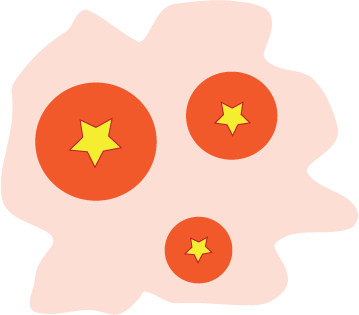
\includegraphics[width=0.98\textwidth]{Figures/CC.png} 
\caption{}
\label{subfig:scenarios:a}
\end{subfigure}
\begin{subfigure}[b]{0.3\textwidth}
\centering
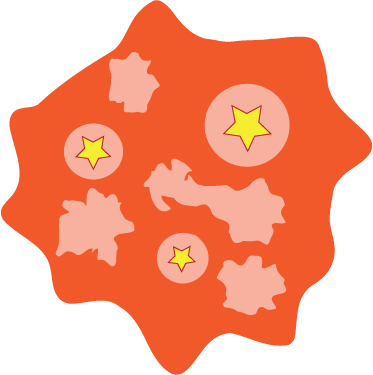
\includegraphics[width=0.98\textwidth]{Figures/CA.png} 
\caption{}
\label{subfig:scenarios:b}
\end{subfigure}
\begin{subfigure}[b]{0.3\textwidth}
\centering
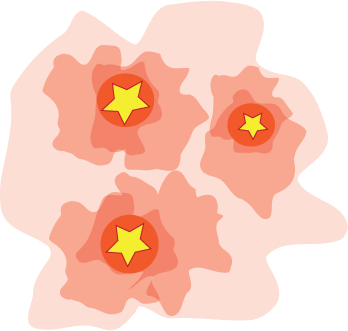
\includegraphics[width=0.98\textwidth]{Figures/Coalescence.png} 
\caption{}
\label{subfig:scenarios:c}
\end{subfigure}
\caption[Scenarios of clustered star formation]{Three scenarios of clustered star formation. Darker colors indicate higher densities.}
\label{fig:SFscenarios}
\end{center}
\end{figure}



%\subsubsection{Outstanding scientific questions}
%Examples: \citep{Hennebelle:2012dk} \citep{Kennicutt:2012ey}
%Ex: WHERE DO THE INEFFICIENCIES COME FROM?
%
%Luminosity problem \citep{McKee:2007bd}
%Angular momentum problem and magnetic flux problem  \citep{McKee:2007bd}
%How the mass-to-flux ratio increases so dramatically during star formation is one of the classic problems of star formation (Mestel \& Spitzer 1956). 

\subsection{Dust as a tracer of star formation}
\label{subsec:dust}

Despite being a small component by mass, interstellar dust is an important component of galaxies. Dust grains are heated up by absorbing the short wavelength emission from stars and re-radiate in the thermal infrared, accounting for $\sim 30\%$ of the total luminosity of the galaxy \citep{Mathis:1990jk}. 

Observationally, dust plays perhaps the most important role when it comes to studying star formation. It usually is assumed that dust is well mixed with the gas, which makes is an excellent tracer of the gravitational well and mass distribution in YSOs. Because H$_2$ and He molecules have very few spectral signatures, they are difficult to observe and study directly. Dust grains block UV and visible star light and emit continuum far-IR radiation, opening a large region of the electromagnetic spectrum for astronomers to study the properties of star formation. Alternative tools to study star formation are dedicated to observing spectral lines of the molecular compounds of the ISM such as CO and other dense gas tracers - a prospect that limits the study to the most dense regions and requires more assumptions to link the abundance of these compounds to the more massive neutral H$_2$ and He gas.


\subsubsection{Dust populations and properties}


Perhaps the first understanding of the composition of dust grains in the ISM was described by \cite{Mathis:1977hp}, where they studied the absorption spectrum of the diffuse ISM, and found that the measurements were appropriately fitted with a dust grain composition of silicates and small graphite particles \citep{Stecher:1965eq}. They were able to fit the observed extinction curve with canonical grain-size distribution, typically $n(a) \propto a^{-3.5}$, where $a$ is the grain size (assuming spherical grains) and $n(a)$ corresponds to the number of grains of sizes $<a$. This assumes low and high cutoffs for the grain sizes, typically \SI{50}{\angstrom} and \SI{0.25}{\micro\meter}, respectively.

This grain-size distribution model was later on enhanced by \cite{Cardelli:1989dp} to account for the difference in interstellar extinctions (hence size distributions) across different galactic lines of sight. These authors were able to successfully parameterize this size distribution using a single parameter, $R_V$, which is the ratio of the total extinction $A(V)$ to selective extinction (or color) $E(B-V)$. Smooth distributions of sizes of graphite and silicate grains between the less dense regions of the ISM, where $R_V = 3.1$, and the dense clusters, where $R_V = 5.3$ \citep{Kim:1994iu}. 

Observations in the thermal infrared from space telescopes have detected strong absorption lines at \SI{9.7}{\micro\meter} and \SI{18}{\micro\meter} which are attributed to stretching mode of Si-O and bending mode of O-Si-O, confirming the presence of silicates in dust compositions \citep{Weingartner:2001du}. Other emission features at 3.3, 6.2, 7.7, 8.6, and \SI{11.3}{\micro\meter} \citep{Sellgren:1994vz} were attributed to bending and stretching modes of polycyclic aromatic hydrocarbons \citep[PAH, see][]{Gillett:1973bh,Allamandola:1985cf}, which are complex, planar organic molecules.
 
A consolidated model matching all-sky measurements by instruments on the COBE space observatory confirms the composition of amorphous silicates and carbonaceous grains with sizes ranging from large grains (\SI{1}{\micro\meter}) down to tens of atoms \citep{Li:2001gk}, where the larger carbonaceous grains have graphitic properties and the smaller population have PAH-like properties.




A large number of dust models exist (see Section~\ref{subsubsec:radiative})


Knowing the dust composition and size distribution of grains is important to properly predict its observational behavior, to relate it to the physical quantities of interest, since the goal of the exercise is to use dust as a tracer of star-forming mechanisms. A given dust model needs to provide several key quantities that can be used in radiative transfer modeling (see Section~\ref{subsubsec:radiative}), such as the albedo, the scattering function, and the opacity.



Talk also about PAHs and VSG to open the door to this topic?
\subsubsection{Interstellar extinction}

Talk about dust properties in the galaxu: \citep{Collaboration:2014dz} Using
\begin{equation}
I_\nu = \tau_\nu B_\nu(T)
\tau_\nu = \kappa_\nu M_\textrm{dust}
\kappa_\nu\propto \nu^\beta
I_\nu = \kappa_0(\nu/\nu_0)^\beta r\mu m_H N_H B_\nu(T)
\end{equation}
Also maybe mention papers by Dale etc DIRBE/COBE

\subsubsection{From dust observations to physical quantities}
Talk about basics (long-wavelength = proxy for mass), and talk about modelling too. Fitting, radiative transfer, etc.

The far-IR luminosity has a number of definitions, and consistency is important in converting them to $M_\star$. A commonly used definition integrates the dust emission over the wavelength range 3–\SI{1100}{\micro\meter} \citep{Dale:2002bo}, and following those researchers, we refer to this as the total- infrared (TIR) luminosity. Note, however, that other definitions based on a narrower wavelength band or even single-band IR measurements are often used in the literature.

\subsubsection{Radiative transfer modeling}
\label{subsubsec:radiative}
Whitney, Robitaille, Wolfire...

\subsubsection{Summary}

Lead this into BETTII

\subsubsection{Observing facilities}


\begin{itemize}
\item \citep{Kennicutt:2012ey} Maybe start with a description of the ISM
\item \citep{Terebey:1984hi} Basics of infall; 
It is well understood how self-gravity can concentrate gas in the presence of magnetic fields, turbulence, rotation, and thermal pressure, leading to protostar formation and accretion ( McKee \& Ostriker 2007; Adams \& Shu 2007; Ballesteros-Paredes et al. 2007)
\item \citep{Adams:1987gy} Spectral evolution of young stellar objects; describe classes of stellar objects, using models and make sure to include size scales; YSO vs protostar
\item Need to mention something about star formation efficiency
\item Need to mention something about outflows and feedback \citep{Maury:2009co}
\item \citep{Larson:1994cj} Molecular cloud characteristics; maybe a good start for text | Give definition of cloud (gravitationally bound in the Virial sense), in terms of number of candidates and stellar mass density (Lada 2003)
\item \citep{Myers:2009fv} It is widely accepted that most stars form in concentrations of dense gas (Beichman et al. 1986), and that such young stars are most frequently found in groups and clusters in molecular clouds (Lada \& Lada 2003). It is less clear how the mass of a protostar is related to the mass of the dense core where it forms.
In one view, a core is essentially a fixed-mass reservoir of gas, which contributes a significant fraction of its initial mass to its protostar. Then core and protostar masses are proportional, and their mass distributions have the same shape (Motte et al. 1998; Alves et al. 2007). Many authors have suggested ways to form a mass distribution of cores which resembles the IMF, particularly from processes of turbulent fragmentation (Hennebelle \& Chabrier 2008 and references therein).
In another view, a core is the densest part of a more extended distribution of gas, with no physical barrier to accretion (Shu 1977; Myers \& Fuller 1992; Caselli \& Myers 1995; McKee \& Tan 2003). Protostars originate in cores, but their masses do not correlate (Bonnell et al. 1998; Bate \& Bonnell 2005), or their correlation depends on fragmentation and core definition (Swift \& Williams 2008), or on the range of gas dispersal times (Myers 2008, hereafter Paper 1). Alternately, their correlation may be coincidental rather than genetic (Hatchell \& Fuller 2008).
\item \citep{McKee:2010iw} Protostellar mass function
\item \citep{Bonnell:1997vta} Accretion in small clusters
\item \citep{Evans:1999gz} Review of physical conditions of star formation, also a good place to start
\item \citep{Myers:2011fy} These results suggest that a simple model is needed for the dense parts of clusters, where protostars start accreting in condensations resembling dense cores, where they can also gain mass from the core environment, where their accretion durations are specified, and where protostar mass is not tied to the gravitational collapse of an isolated initial condensation. | This comparison favors the core–clump model over the isolated core model for star formation in embedded clusters. It suggests that initial core structure need not set protostar mass, and that massive stars are clump-fed.
\item Clusters are laboratories for studying a wide range of astrophysical phenomena; stars of large range of masses which are formed roughly simultaneously (Lada 2003), can understand stellar evolution theories; 
\item \citep{Lada:2003il} Cluster formation within molecular clouds: Because a cluster is held together by the mutual gravitational attraction of its individual members, its evolution is determined by Newton's laws of motion and gravity; |
Stars form in dense gas; therefore, it is not surprising that a high fraction of all stars form in highly localized rich clusters because most of a cloud’s dense gas is contained in its localized massive cores.; |
This would suggest that there is a direct mapping of clump mass to stellar mass and that the substructure of cluster-forming cores reflects the initial conditions of the star-formation process in dense cores. |
The structure of an embedded cluster is of great interest since it likely possesses the imprint of the physical process responsible for its creation. In particular, structure in the youngest embedded clusters reflects the underlying structure in the dense molecular gas from which they formed. | A fundamental consequence of the theory of stellar structure and evolution is that, once formed, the subsequent life history of a star is essentially predetermined by one parameter, its birth mass
\item \citep{Bate:2003cv} Evolution of clusters (dynamics, showing simulations and such); same as \citep{Bonnell:2003iw}; realte to potentially having multiple generations of stars within the same cluster; \citep{Allen:2007wqa}
\item \citep{Mathis:1990jk} Pioneering paper on the interstellar extinction by dust
\item \citep{Weingartner:2001du} Paper on dust populations
\item \citep{Li:2001gk} Very small grain population and non-LTE heating
\item \citep{Compiegne:2010kk} Large surveys, PAHs, VSG, etc
\item \citep{Bastian:2010ig} Big picture: importance to universal IMF
\item \citep{Kennicutt:2012ey} The Challenge of Spatially Resolved Star-Formation Rates in Galaxies
\item \citep{Hennebelle:2012dk} Observational issues: 

\end{itemize}



%How do stars accrete their material in dense, clustered environments? Multiple theories have been put forth to explain the forces at play in these important regions of stellar birth \citep[e.g.][]{Bonnell:1997vta, McKee:2003gxa}. Pivotal differences in the theories center around what drives the parsec-scale dense cloud to form many stars and how the forming stars acquire their mass. Does dense gas fragment into isolated centers of collapse? Are turbulent motions in the gas driving creation of super-critical cores? Do young stars competitively accrete material from a surrounding common reservoir? Do gravitational interactions between forming young objects play a significant role in setting the final stellar mass function? Better observational understanding of these clusters is necessary to address these questions and to discriminate between the different models, as noted by \cite{Bonnell:2006ee}, \cite{Offner:2011ex} and \cite{Myers:2011fy}.
%
%\textbf{The primary goal of the proposed science plan is to understand how stars accrete material on the scales of 100's to 1,000's of AUs in forming cluster cores}. Given the typical stellar separations in clusters with fully formed young stellar objects (YSO) and the typical densities of gas in these cores, 1,000's of AUs are the size scales over which forming stars must draw material to become 0.5-10 solar masses. Once the material is inside 100 AU, it is strongly bound to the forming stellar system (which may be one or more stars) and its fate is determined. To give an idea of the possibilities for accreting material, Fig. \ref{fig:SFscenarios} sketches three scenarios for how stars could capture mass in the cluster environment: core collapse, competitive accretion, and collisional merging. In core collapse \citep[Fig.~\ref{scenarios:a},][]{McKee:2003gxa, Myers:2011fy}, the cluster's gas fragments into cores which collapse individually to form single, binary, or small multiple star systems; the available mass is defined by the original fragment. In competitive accretion \citep[Fig.~\ref{scenarios:b},][]{Bonnell:1997vta}, the initial core collapses but contains a small fraction of the star's final mass; additional mass is captured competitively with other forming stars from the surrounding dense core gas. In collisional merging \citep[Fig.~\ref{scenarios:c},][]{Bonnell:2002et}, the initial fragments interact gravitationally and form larger mass cores before and during the formation process. 
%
%Are all these processes observed at once in star forming clusters? What conditions favor one versus the other, and why? Are these processes observed at different stages in the cluster's history? These questions need more observational data to be answered. \textbf{We propose to gather information about the gravitational potential within the cluster, the distribution of the turbulence, and the gas densities} \citep{Bonnell:2006ee}. This will advance the problem to the next stage and help answer some of these questions.
%


%\subsection{The physics of star formation}
%
%In here, describe the basics of star formation; include state-of-the art dynamical modeling, radiative transfer modeling, SED fitting, etc.
%
%\subsubsection{Dust populations}
%
%About how to estimate the mass
%
%\subsubsection{Geometry and model degeneracies}
%
%\subsubsection{Foreground extinction}
%
%\subsection{Clustered environments}
%
%\subsubsection{Observational challenges}
%
%Surveys vs pointed observations; show why BETTII is important using IRAS20050's example;
%
%\subsubsection{Observing facilities}
%
%Spitzer, Herschel, SOFIA; radio interferometers;

\section{The Balloon Experimental Twin Telescope for Infrared Interferometry}

\subsection{Towards higher angular resolution in the far-IR}
Observations at mid- to far-infrared wavelengths from the Earth's surface are extremely 
limited by the large atmospheric opacity in this region of the spectrum. Space-based telescopes 
like IRAS \citep[12-100 \um;][]{1984ApJ...278L...1N}, ISO \citep[2.5-240 $\um$;][]{1996A&A...315L..27K}, \textit{Spitzer} \citep[3.6-160 $\um$;][]{2004ApJS..154....1W}, AKARI  \citep[1.7-180 $\um$;][]{2007PASJ...59S.369M}, WISE \citep[3.4-22 $\um$;][]{2010AJ....140.1868W} and \textit{Herschel} \citep[55-672 $\um$;][]{2010A&A...518L...1P} have demonstrated the scientific value of observations at 
these wavelengths; but the spatial resolution of space-based observatories is limited by the cost 
and complexity of building and flying progressively larger aperture telescopes. 

In this work, we discuss progress in understanding clustered star formatino through increased angular resolution, by using SOFIA and BETTII, both operating at high altitudes in the atmosphere. High--altitude observatories are a good compromise between ground and space observatories: while less sensitive because of the surrounding thermal emission from the atmosphere, they can still feature larger optics, more experimental setups, and instrumentation that can be changed on a more frequent basis.

SOFIA has a \SI{2.7}{\meter} primary mirror which is a significant size improvement over \Spitzer. The instrument we have used, FORCAST, provides unprecedented high angular resolution of \ang{;;2}-\ang{;;3.5} in multiple continuum bands from \SI{5.5}{\micro\meter} to \SI{37.1}{\micro\meter}, which allows us to probe a relatively unexplored region of phase space.

BETTII is an experiment that aims at breaking from the single-aperture paradigm by using interferometry between 30 and \SI{90}{\micro\meter} from a balloon platform. Interferometry is commonly used on the ground at other wavelengths such as optical and radio, and is a viable path forward to obtain much higher resolution than what single apertures can provide. 

In this work we focus on the particular technique called \textit{spatio-spectral interferometry} \citep{Mariotti:1988vea}, which is a way to achieve 
high angular and moderate spectral resolutions at far-IR wavelengths from above the atmosphere, without the cost and limitations of large single apertures. 


\subsection{The stratospheric balloon environment}

Mention briefly the conditions at balloon altitude: temperature, pressure, cosmic rays, pendulum modes; required shock resistance; picture of the launch; 


\subsection{BETTII description}

%The Ballon Experimental Twin Telescope for Infrared Interferometr (BETTII) project is pioneering a new technique that could lead to dramatically increased spatial resolution in the far-infrared: spatio-spectral interferometry. 
As a cryogenic payload flying at an altitude of \SI{37}{\kilo\meter}, BETTII is the first flying "direct detection" interferometer: it will attempt to coherently combine light from two different telescopes to provide increased angular resolution. Because it is operating from above the atmosphere, it can see the far-infrared universe between 30 and 90 \si{\micro\meter}, and provide \ang{;;0.5}-\ang{;;1} spatial resolution at these wavelengths - a key region of parameter space well-suited to study protostars evolving in dense clustered environments.

To provide this resolution which matches that of \JWST  at \SI{25}{\micro\meter}, BETTII needs to be have two collectors separated by $\approx$\SI{8}{\meter}; Because of its operating wavelength, it needs to have a cryogenic instrument; because it is an interferometer, it needs optics with exquisite surface quality; and because it flies on a balloon platform, it needs to be robust to large changes in temperature, large pointing errors, and severe shock resistance for the landing phase.

Throughout this chapter, we will first discuss the basics of double-Fourier interferometers, before presenting the general design of BETTII payload and most of its subsystems.


\subsection{Basics of interferometry}

Since the end of the 19th century with Michelson [reference], scientists have learned how to use the wave properties of light to learn about new astrophysical phenomena. It did not take long for what first started as a laboratory experiment by Michelson and Morley [cite] to be applied to astronomy, with Michelson Stellar Interferometer experiment. 

The principle of interferometry is simple. Because light behaves like a wave, two beams of light coming from the same source can be combined \textit{coherently}, provided that their amplitudes and phases are controlled. The intensity of the combined signal is a function of a) the brightness of the light beam, but also b) the relative phase and wavefront of each beam, which can create a modulation of that brightness.

Michelson and Morley created what became the standard Michelson interferometer. It uses one single source of light and a beam splitter that creates two coherent light beams from that one source. The two light beams go through two separate \textit{arms} before being recombined. While adjusting the length of one arm with respect to the other, we modulate the phase difference between the two arms, leaving everything else the same. This creates a modulation called an \textit{interferogram}, which describes the measured intensity variation as a function of the phase difference between the two arms.

The phase difference is expressed in radians and depends on the wavelength of the light that is used. In this work, we will usually refer to this difference in terms of an actually physical distance instead: the optical path difference (\OPD). This has the advantage of being wavelength-independent and relate more easily to opto-mechanical considerations.

[image of a standard Michelson interferometer]

[Explain here the combination of two monochromatic beams]


\begin{figure}[!ht]
	\centering
	\includestandalone[width=\textwidth]{Figures/interferogram}
	\caption[Simple interferogram]{An ideal interferogram here is shown as a sum of cosine waves of different frequencies.}
	\label{fig:interferogram}
    \end{figure}

\subsubsection{Fourier transform spectroscopy}

One immediate consequence of the original Michelson experiment is to realize that the interferogram actually contains spectral information. For an ideally monochromatic source, the intensity modulation (or \textit{fringe}) depends on the \OPD only modulo a wavelength. This means that the modulation is identical whether we introduce an $\OPD = \lambda$, or $\OPD = n\lambda$, where $n$ is an integer. This is because the monochromatic wave can essentially be represented by an amplitude times a cosine function of phase (or a cosine function of $2\pi\OPD/\lambda$).

The intensity of modulation for a given wavelength is then a cosine wave as well, with an amplitude related to the intensity of the signal, and a wavelength equal to the wavelength of the incident light.

If we consider a polychromatic signal as a sum of monochromatic wavelengths, this phenomenon happens for each single wavelength, and the resulting intensity modulations add \textit{coherently}: the total intensity is the coherent sum of the intensity modulations created by each individual wavelength. This has the effect of smearing the resulting modulation in most places except around the precise location where the \OPD is zero. Around this location, the modulation is not wavelength dependent, and fringes are always seen. These are commonly referred to as \textit{white light fringes}. The range of wavelengths in which fringes can be seen is called the \textit{coherence length} \Lc. When all wavelengths are weighted equally in a bandpass $\Delta\lambda$, the coherence length can be expressed as:
\begin{equation}
\Lc = \frac{\lambda^2}{\Delta\lambda},
\end{equation}
and the interferogram can be represented by a carrier frequency modulated by an envelope function:

[add equation for the integral of interferograms]
%\begin{equation}
%\sum_{\lambda_i}\I_i = \frac{\lambda^2}{\Delta\lambda},
%\end{equation}

Since the modulation is a coherent superposition of cosine waves, it contains spectral information. A cosine transform of the interferogram will decompose the contribution of each individual wavelength, hence reproducing the spectrum of the polychromatic source. This realization has led to many scientific discoveries in astronomy, chemistry and other fields over the last 100 years.

[Add picture of Mach-Zehnder testbed from second year project]

\subsubsection{Aperture synthesis}


\begin{figure}[!ht]
	\centering
	\includestandalone[width=\textwidth]{Figures/interferometer}
	\caption[Michelson Stellar interferometer]{A Michelson Stellar interferometer.}
	\label{fig:interferometer}
    \end{figure}


An interferogram is produced by coherently combining photons from one single source of light. This can be applied for example for an infinitely far astronomical source: as the light propagates from the source, by the time it reaches our instrument the radius of curvature of its wavefront is extremely large, and the latter can be approximated as being flat. The photons from this source nominally enter each arm of the interferometer with the same phase, when the alignment is perfect. When combined, these photons would interfere and create an interferogram.




However, let's suppose that a second source is sufficiently far away from the first source that its wavefront enters the interferometer at an angle. This means the photons from the second source enter one arm slightly later than the other - or that photons need to cross more optical path in one arm than in the other. These photons would also create an interferogram, but the latter will be centered about a different position in \OPD  space than the interferogram created by the photons from the first source. Now let's suppose that the second source is exactly as bright as the first one, and that it is apart from the first by an angle $\theta$ such that $\baseline\sin\theta = \lambda/2$. In this case,  the interferogram created by the photons from the second source has the same amplitude as the first interferogram, but is shifted by half a wavelength in \OPD. As a result, the two interferograms would exactly cancel each other, and we would say that the \textit{spatial degree of coherence} between the two sources is zero. Although the sources are not coherent in the strict sense because they are completely independent sources, the intensity modulation (or interferograms) caused by each source would, in this case, cancel out. If the angular separation was such that $\baseline\sin\theta = \lambda$, then the modulations would add up and the resulting modulation would have twice the amplitude of that with just one single source. We would say that the spatial degree of coherence between the two sources is unity. 

\begin{figure}[!ht]
	\centering
	\includestandalone[width=\textwidth]{Figures/aperturesynthesis}
	\caption[Aperture synthesis]{Relevant planes in the optical train for aperture synthesis.}
	\label{fig:aperturesynthesis}
    \end{figure}



One way to formalize this important property is to consider an interferometer with a given baseline length and angle as a filter of the source's spatial distribution on the sky. For a given baseline length and angle with respect to the sky, the interferometer is only sensitive to a single angular frequency in a single direction on the sky. Various sources observed simultaneously by the interferometer will all contribute to a single measured interferogram (or intensity modulation), which can be characterized in terms of the spatial degree of coherence, also called \textit{complex visibility}, between the sources for a given baseline angle and length. 

The generalization of this property is called the Van Cittert-Zernike theorem: the 2D Fourier transform of the intensity distribution on the sky is its complex visibility function. In other words, by mapping the complex visibility (through measuring interferograms) for all baseline angles and lengths, we can reconstruct the original image through an inverse Fourier transform. The plane of complex visibilities is commonly referred to as the (u,v)-plane [CITE THOMPSON 2008].





Pictures:
\begin{itemize}
\item Show source plane, u,v plane, baseline sampling, and image plane
\item Picture of single wavelength interferogram (use Python to generate values, and tikz to display?)
\item Picture of multi-wavelength interferogram, with envelope, etc.
- Optics diagram of two-aperture Michelson interferometer FTS vs single-aperture FTS
- picture of the interferometer as a spatial filter on the sky
\end{itemize}

Watch out, we are being redundant with chapter 2. what do we do?

\subsubsection{Double-Fourier interferometry}

Interferometry and aperture synthesis is used commonly at radio wavelengths, where coherent detectors can obtain the direct phase of the incoming light by mixing the signal with a local oscillator. Both the amplitude and the phase of the signal can be recorded for each antenna, and can be combined with all the other antennas at a later time.

Aperture synthesis has also been achieved at optical and near-infrared wavelengths, where a nearby guide star is used to determine a reference phase of the incoming beam. The fringe patterns measured for the science sources can then be non-ambiguously aligned with each other. This process requires very rapid imaging capabilities (on the order of \SI{10}{\milli\second}, a typical atmospheric coherence timescale) to freeze the atmospheric variations across the synthetic aperture. This requires bright guide stars. In addition, because of the large baselines, the field of view is very limited, so the targets accessible by optical interferometers are limited to scientific sources which are a few arcseconds of a bright guide star: this dramatically limits the capabilities of ground-based interferometry at these wavelengths.

In the far-infrared, coherent-detection interferometers are a possibility [ESPRIT], but they presently lack sensitivity and may be fundamentally less efficient than direct-detection arrays. In this work, we take advantage of recently-developed Transition Edge Sensor bolometer arrays, which are direct-detection, power sensors (which means that we do not have access to the phase information). Hence phase referencing during flight will have to be achieved very carefully.

We adopt a Michelson interferometer configuration that we use in pupil-plane combination. Unlike image-plane combination, where fringes are seen across a single Airy disk in the image plane, no fringes are visible across the field of view for a given \OPD. Instead, the intensity of the entire field of view is modulated as a function of \OPD. 

By scanning the \OPD, we obtain a modulation of each pixel on the detector, which combines information on both the spectral (through the Fourier transform of the scan) and the spatial (through the amplitude of the fringe packet) content of the source, at that baseline orientation and length. By repeating the measurement over multiple baseline angles and lengths, one can unambiguously retrieve both the spatial and spectral content of the astronomical scene. 

Pupil-plane combination allows for an interferometric response of the entire field of view. The price we pay is that the \OPD scans need to be longer in order to cover enough spectral range for each pixel in the field of view. For a single-pixel detector, the \OPD scan would only need to cover enough stroke to obtain the desired spectral resolution over that one single pixel.


\subsection{BETTII Instrument design}

Mention that we cover the control system in detail in chapter 3.

\subsubsection{Overview}

The BETTII payload is an \SI{8}{\meter} fixed-baseline interferometer, equipped with 2 \SI{50}{\centi\meter} siderostats. It operates in two wavelength bands, 30-55~\si{\micro\meter} and 55-90~\si{\micro\meter}. In these two bands, its theoretical angular resolution is \ang{;;0.5} and \ang{;;1}, respectively. This is significantly better than all existing or previous facilities that operate in the far-infrared, which have traditionally been limited by the mirror size. In addition, this matches the resolution of JWST at \SI{25}{\micro\meter}, hence providing a good continuity to probe astrophysical phenomena at longer wavelength but with the same linear resolution.

[Put table of aperture size and angular resolution of all large space missions].

There are four major components to BETTII: the mechanical structure and design; the optics and their mounts; the cryostat and the detectors; and the control system. The latter will be discussed extensively in chapter \ref{chap:controls}. In this section, we will introduce the three other aspects of the BETTII payload.

[Make table with primary characteristics]

\subsubsection{Stratospheric balloon environment}

High-altitude balloons have for many years served as a test platforms for future space instruments, such as COBE. These balloon platforms fly between 30 and \SI{40}{\kilo\meter}, above more than 99\% of the atmosphere, which make them particularly well suited for studying the universe at infrared, far-infrared and sub-millimeter wavelengths. Balloon launches occur year-round across all continents, including Antarctica, which allows balloon flights that can last for multiple weeks. 

For a typical launch, the scientific payload is attached on the bottom of a train of about \SI{100}{\meter} that includes a parachute and a ladder. The top of the ladder attach to the bottom of the large helium-filled balloon. 

[Put picture of balloon launch]

At float altitude, the air temperature is between \SI{230}{\kelvin} and \SI{250}{\kelvin}, while the air pressure is down to 0.5\% of the sea level pressure (about 5 mbar). Upper altitude winds are large-scale laminar flows that move the balloon and the payload as one. This can excite pendulum motions about the pivots underneath the balloon and at the top of the payload, which are typically of the order of a few arcminutes and have periods of a few to many tens of seconds [cite FIXSEN]

The payload's temperature and temperature distribution is influenced by the air temperature, the infrared radiation of the Earth, and the sunlight, which can result in complex temperature gradients across the instrument. A better temperature uniformity is expected for night flights, which is what BETTII is expecting.

Balloon experiments can also be affected by cosmic rays which can damage the electronics, lead to data corruption and or failures of the software/control system. However, this becomes more of an issue for long-duration balloon flights around Antarctica, during which the payloads are exposed for many weeks to the cosmic ray environment.

BETTII is expected to launch from Fort Sumner, NM, for its first engineering flight. After a morning launch, we expect to wait until nightfall to achieve proper thermal stabilization and achieve our science goals. We expect the flight to last about \SI{16}{\hour}, although this is highly dependent on the weather and wind patterns.


\subsubsection{Mechanical design}

BETTII has two main structures. The first is a carbon fiber and steel truss that is used as our optical bench. This was the first item that was designed in the project. The elements of this structure are built by bonding \SI{7.5}{\centi\meter} carbon tubes to custom-made steel nosecones. The steel nosecones are lightweight and strong, and have a threaded hole on the axis: they attach to multi-faceted steel nodes like tinker toys. There are three lengths of tubes on the truss. At the interface between the nosecone and the nodes, spherical washers or polypropylene washers are used, depending on the location on the payload. The difference of material compensates for differential thermal contraction on the beams that form the long side of triangles.

The structure is about \SI{9}{\meter} long. It is designed to be lightweight, strong, and have a first resonant mode above \SI{20}{\hertz} to ensure fast damping of residual mechanical oscillations. This property was measured and the predicted resonance was found to be within \SI{1}{\hertz} of its expected frequency, at \SI{25}{\hertz}.

The strength of each bonded tube assembly was also tested. Each assembly was individually subject to a \SI{10000}{\newton} pull test. Out of all the assemblies [FIND NUMBER], only 2 failed close to \SI{10000}{\newton}, at the level of the epoxy bond. 

The entire balloon payload needs to be robust to handle 10~g vertical force and 5~g force at \SI{45}{\deg}. With an expected total mass of \SI{1000}{\kilo\gram}, we need yield strength sufficient to hold \SI{100000}{\newton} of force. 

The gondola is what holds the truss and attaches to the balloon train. It also holds the electronics, reaction wheels, batteries, and communications to the ground. The frame is made out of 80/20 T-slotted aluminum bars that are attached together using T-inserts, and reinforced by screwed-on corner plates. The precision of this payload is of no importance to the optical alignment. 

The various electronic components of the system are attached to the gondola using aluminum or honeycomb aluminum plates, which are painted with white appliance paint for better thermal behavior. These plates act as radiator panels which allow us to dissipate the heat out to space.

The most critical portion of the gondola is the assembly that connects to the balloon train. This holds a single pin that needs to have the highest yield strength, since it is the only point of the payload that needs to support the entire weight. A more detailed description of the pin is presented in Section~\ref{subsec:chap3momdumpmotor}.



\subsubsection{Warm optical system}

The optical system was one of the most challenging design aspects of the project. It is beyond the scope of this work to go into details about all the considerations that went into the design, but we will review some of the main aspects: the overall optics layout, and the fabrication of the telescope assemblies.

\paragraph{Optics layout}
Because the nature of balloon payloads, there can be extensive damage to the structure during parachute opening and landing. In order to minimize the repair costs from one flight to the next, it was decided to place the telescope assemblies - which are expensive, long lead-time items - away from the edges of the truss. 

Instead, flat mirrors are used to redirect the light towards the telescope assemblies, which are kept close to the center of the truss where damage is expected to be minimal. 

The telescope assemblies consist of 3 powered mirrors and a folding flat. They provide a 20:1 compression ratio of the beams with reasonable tolerance on the mirror positioning. As an all-aluminum assembly, they shrink homologously as the temperature varies during the different phases of the flight, hence maintaining optical prescriptions. 

In order to perform double-Fourier interferometry, an asymmetry needs to be introduced in the system in order to properly combine the polarizations of the light at the beam combiner. This asymmetry occurs after the telescope assemblies and before entering the cryostat. In one arm, a 3-mirror assembly (called the K-mirror assembly, or KMA) is used on a rotating stage to properly de-rotate the field of view as the telescopes change elevation. On the other side, a 4-mirror delay line assembly (called the Warm Delay Line, or WDL) is set at a fixed orientation. Its role is to compensate for the optical delays caused by the residual pointing errors. 

On both the KMA and the WDL, on of the mirrors is actuated in tip and tilt, and provide the fine control required to properly overlap the two beams [discussed in section...]

[Show picture of the optics train]

The beams of light enter the cryostat through a thin polypropylene window. We tested different window thicknesses and selected the \SI{15}{\micro\meter} thickness as our baseline design. Test pieces with this window have been shown to comfortably resist about 1.5 times the atmospheric pressure, even after 50 cycles of pressurization. The number is a little smaller when the pressurization occurs very rapidly and do leave time to the window to deform elastically. A number of tests were done on identical batches of windows to ensure the repeatability of our test method. 




\paragraph{Optics manufacturing}

Despite working at relatively long wavelengths, the tolerance in the surface figure of all the mirrors is an important consideration. Traditionally, figure errors are specified in terms of the required beam quality at in the focal plane, which starts to degrade when the wavefront errors in the optical train are comparable with the wavelength of the light beam, or introduce specific aberrations such as coma. In interferometers, the fidelity of the final image is not a priority. However, differential wavefront errors between the two optical trains before combination will result in decreased contrast of the interferograms. As a result, the surface quality of the mirrors pre-combination needs to be much lower than a wavelength of light, since errors will stack after hitting many mirrors from both sides. For our specifications, we determine that a \SI{300}{\nano\meter} r.m.s surface figure error over the entire aperture is sufficient to ensure decent scientific results. This requirement is difficult to match for the largest elements in our optical train (the siderostats and the primary mirror) - but smaller mirrors pose less of a challenge in their manufacture. It is important to mention that figure errors are a concern for us because we are using all-aluminum optics, as opposed to more traditional materials such as glass which are easier to polish.

The company Nu-Tek, in Aberdeen, MD manufactured all of our small optics out of aluminum. The procedure includes an initial milling process, heat treatment, followed by diamond turning and gold coating to avoid oxidation.

However, very few manufacturers in the United States were able to diamond-turn the siderostats and the primary mirror assembly, while ensuring the level of surface figure we needed. The diamond-turning process uses a slowly moving diamond blade that is controlled in 3 axes to carve out the required shape. This process requires extreme temperature stability, which is often not available in traditional machine shops. 

The Department of Advanced Manufacturing at North Carolina State University was able to manufacture our mirrors by meeting all of our requirements. The results are published in [REF to JATIS paper]. Each telescope assembly has a stacked RMS surface figure error of [], while the siderostats have []. The siderostats are more complicated because they did not exactly fit in their diamond-turning spindle. We decided to proceed with a two-step diamond turning, where they turned two sections of the ellipse consecutively. This does not guarantee that the two areas will be at the same height since they have to unmount the mirror off the spindle. However, our models show that even if different sections of the mirrors are at different heights, the beam combination can still be successful, as the parts of the pupil that are shifted in one arm are also shifted in the other. 




\subsubsection{Cryogenic instrument}

The cryostat was design by our team. Items were sent out for manufacturing to different companies and assembled in house. The cryostat is passive and does not require any mechanical cryo-cooler. It is designed to operate for a duration of \SI{40}{\hour}, which should give us enough margin considering the typical lengths of balloon flights from the U.S. of about \SI{16}{\hour}. 

The fridge is a ($^3$He+$^4$He) sorption refridgerator from Chase Research that cools down the main optical bench to \SI{4}{\kelvin}. It also has an intermediate cold finger at \SI{1}{\kelvin} and a final stage that brings down the detector temperature to \SI{300}{\milli\kelvin}. 

At the heart of the instrument are four $9\times 9$ close-packed linear arrays of multiplexed superconducting transition edge sensors (TES) bolometers [REF Benford et al. 2008] incorporating the Backshort Under Grid (BUG) architecture [REF Allen et al. 2006]. These arrays are scaled versions of similar arrays already built for ground-based instruments (e.g., GISMO: REF Staguhn et al. 2006, 2014). Detectors are read out using advanced linear SQUID multiplexer and amplifiers. A $4\times 22$ multiplexed readout is used for each array; the extra seven channels are used for calibration signals (unilluminated pixels, “dark SQUID” channels, and an “always on” channel), allowing monitoring of all potential noise contributors [REF de Korte et al. 2003].  

The optics inside the cryostat include two sections: a near-infrared fine guidance sensor, and the far-infrared channels which lead to the science detector. The incoming light beam is split right after entering the cryostat with a NIR/FIR dichroic beam splitter. This custom-made filter reflects off the far-IR and transmits the near-IR, and its recipe was suggested by P. Ade at Cardiff University. At the bottom of the cryostat, in the \SI{77}{\kelvin} volume, the fine guidance sensor is composed of N optics and one H1RG detector [REFERENCE]. 

At the top of the cryostat and attached to the \SI{4}{\kelvin} cold plate, there is a cold optics bench that holds all of the far-IR optics, filters, and the Cold Delay Line. All filters were manufactured by Cardiff University in the U.K. The layout of the optical system is shown in Figure [], and more details can be found in [REF ARNAB's SPIE PAPER].



\subsubsection{Data products \& analysis}


Once in flight the payload operations consist of pointing at a target, stabilizing the attitude motions, and scanning the delay while recording detector data. A number of operational modes are required to ensure we reach this stable observing stage, and are described in more details in section [REF]. 

Individual scans will last for a nominal duration of \SI{3}{\second}, and consist of \si{1024} individual detector frames, which are matched to a given \OPD. To increase the signal-to-noise ratio (\SNR), we expect to stack \SI{10}{\minute} worth of data, which corresponds to 200 scans. For this duration, we expect that the change in the baseline angle due to the rotation of the Earth is negligible. It is critical to correctly stack the interferograms, as \OPD errors from scan to scan can significantly reduce the fringe contrast (see [CHAPTER 2]).

To describe post-processing, let's consider a \SI{10}{\minute} cube which is the {\OPD}-corrected stack of images from the 200 individual scans. The cube has a crossection of $9\times 9$, and a depth of 1024 frames. For each frame, the intensity of each source in the detector is determined for each \OPD, and combined into interferograms. We repeat the process for the same field observed at different baseline angles. 

The set of cubes are fed to an inversion algorithm that was developed in Dr. Juanola-Parramon's Ph.D. thesis [REFERENCE], which provides a final datacube corresponding to the images as a function of wavelength, with the spectral resolution that the user chooses. 

\begin{figure}[!ht]
	\centering
	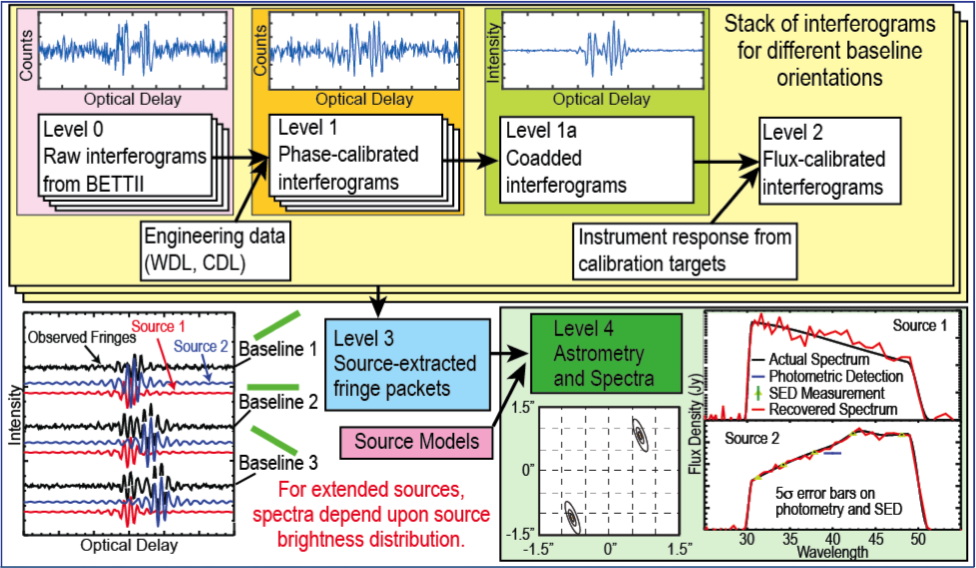
\includegraphics[width=\textwidth]{Figures/DataProcessing.png}
	\caption[Data processing]{BETTII data processing steps.}
	\label{fig:dataProcessing}
    \end{figure}




\subsection{Sensitivity analysis}

Early in my involvement with BETTII, I led the effort in trying to estimate the sensitivity of our instrument, in order to select relevant scientific targets, but also find astronomical calibrator objects which would help us understand the systematics of our payload.

In this section, we summarize our findings and give details on the methods and equations we used. Since only very few authors have approached the problem of double-Fourier interferometers, we were able to derive a new formalism to estimate the spectral sensitivity of double-Fourier interferometers for point sources. Our method uses propagation of gaussian errors through Fourier transforms, and is described in detail in Chapter~\ref{chap:phasenoisepaper}. This can be useful to determine the sensitivity of other types of instruments, such as a space-based follow-up of BETTII, which we briefly discuss in the conclusion of this work.

\subsubsection{Instrument and observing parameters}

Table~\ref{tab:instrumentParameters} represents the key instrument parameters that are relevant for the sensitivity estimation of the two science channels of BETTII. Some of these parameters are user inputs (such as the aperture size), and some are already derived. A detailed, custom calculator tool uses a few user inputs to provide a number of instrumental properties, which in turn serve as design baseline for various subsystems. For example, the "OPD range required" is a derived output, depending on the baseline length, the field of view and the required spectral resolution.

\renewcommand{\arraystretch}{1.5}
\setlist[itemize,1]{nolistsep,leftmargin=*,labelsep=-\mylen}
\def\labelitemi{--}
\begin{table}[htbp]
\small
\begin{longtable}{P{6cm}|c|c|P{1.5cm}}
\toprule											
Parameter	&	\multicolumn{2}{c|}{          		 Value		} 			&	Units	\\
\midrule											
Input aperture	&	\multicolumn{2}{c|}{		0.196		}			&	\si{\raiseto{2}\meter}	\\
Baseline length	&	\multicolumn{2}{c|}{		8		}			&	\si{\meter}	\\
Detector pixels	&	\multicolumn{2}{c|}{	$	9\times 9	$	}			&	pixels	\\
Integration time per full frame	&	\multicolumn{2}{c|}{		2.5		}			&	\si{\milli\second}	\\
Nominal scan speed	&	\multicolumn{2}{c|}{		2.73		}			&	\si{\milli\meter\per\second}	\\
OPD range required	&	\multicolumn{2}{c|}{		8.2		}			&	\si{\milli\meter}	\\
Number of data points in one scan	&	\multicolumn{2}{c|}{		1024		}			&	points	\\
Time per u,v point	&	\multicolumn{2}{c|}{		10		}			&	\si{\minute}	\\
\midrule											
	&		Band 1		&		Band 2		&		\\
\midrule											
Central wavelength	&		40		&		82		&	\si{\micro\meter}	\\
Etendue per pixel	&	\num{	8.2E-10	}	&	\num{	1.8E-09	}	&	\si{\raiseto{2}\meter\steradian}	\\
Required spectral resolution	&		10		&		10		&	$\lambda/\Delta\lambda$	\\
Pixel angular size	&		13.32		&		19.72		&	\si{\arcsec}	\\
Full width half max	&		17.31		&		35.49		&	\si{\arcsec}	\\
Field of view	&		2.00		&		2.96		&	\si{\arcmin}	\\
Number of samples per fringe	&		4		&		8.2		&		\\
\bottomrule											
\end{longtable}
\caption[Instrument parameters]{Instrument design parameters for BETTII.}
\label{tab:instrumentParameters}
\end{table}

\subsubsection{Far-IR background noise estimation}

We proceed to an estimation of the background noise contributors. In Table~\ref{tab:noiseparams}, we list the main sources of noise which can be attributed to bodies in thermal equilibrium. By far the strongest contributors are the warm optics and the cryostat polypropylene window.

In addition to the noise of our own system, we need to take into account the noise generated by the atmosphere, which results in a more complex calculation. For best accuracy, we use quantities from \cite{Harries:1980cva}, who measured the actual sky radiance in a large range of wavelengths from balloon altitudes. We obtain a radiance of \SI{0.16}{\watt\per\raiseto{2}\meter\per\steradian} and \SI{0.07}{\watt\per\raiseto{2}\meter\per\steradian} for band 1 and 2 respectively. This corresponds to \num{2.6e10}~photons~\si{\per\second} and \num{5.2e10}~photons~\si{\per\second}, respectively. 


\begin{figure}[!ht]
	\centering
	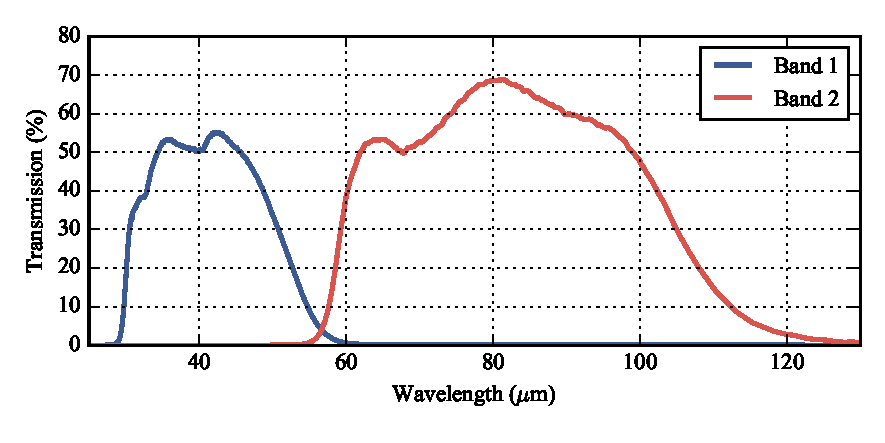
\includegraphics[width=\textwidth]{Figures/BETTII_transmission.pdf}
	\caption[BETTII Transmission curves]{BETTII Transmission curves.}
	\label{fig:aperturesynthesis}
    \end{figure}


\renewcommand{\arraystretch}{1.5}
\setlist[itemize,1]{nolistsep,leftmargin=*,labelsep=-\mylen}
\def\labelitemi{--}
\begin{table}[htbp]
\small
\begin{longtable}{p{3cm}ccP{2cm}P{2cm}p{3cm}}
\toprule
Noise source	&		T (K)		&		Emissivity		&		Photons~\si{\per\second} Band 1		&		Photons~\si{\per\second} Band 2		&	Reference	 \\
\midrule
Warm optics	&	\num{	240	}	&	\num{	0.1	}	&	\num{	1.38E+11	}	&	\num{	9.97E+10	}	&	Assumes 99\% per mirror	\\
Window	&	\num{	240	}	&	\num{	0.02	}	&	\num{	2.76E+10	}	&	\num{	1.99E+10	}	&	Lab measurements	\\
Zodi dust	&	\num{	245	}	&	\num{	3.00E-07	}	&	\num{	2.92E+05	}	&	\num{	3.41E+05	}	&	\cite{Fixsen:2002da}	\\
Galactic Cirrus	&	\num{	20	}	&	\num{	1.23E-04	}	&	\num{	1.79E+01	}	&	\num{	7.67E+04	}	&	\cite{Bracco:2011gw}	\\
Zodi scattering	&	\num{	5800	}	&	\num{	1.00E-13	}	&	\num{	1.47E+01	}	&	\num{	1.31E+01	}	&	\cite{Fixsen:2002da}	\\
CIB	&	\num{	18.5	}	&	\num{	1.30E-05	}	&	\num{	2.19E+00	}	&	\num{	9.68E+03	}	&	\cite{Fixsen:1998br}	\\
Instrument	&	\num{	4	}	&	\num{	0.7	}	&	\num{	5.80E-27	}	&	\num{	2.50E-07	}	&	Estimate	\\
CMB	&	\num{	2.728	}	&	\num{	1	}	&	\num{	1.02E-45	}	&	\num{	9.35E-17	}	&	\cite{Fixsen:1996di}	\\
\bottomrule
\end{longtable}
\caption[Thermal noise contributors]{Thermal noise contributors.}
\label{tab:noiseparams}
\end{table}

\renewcommand{\arraystretch}{1.5}
\setlist[itemize,1]{nolistsep,leftmargin=*,labelsep=-\mylen}
\def\labelitemi{--}
\begin{table}[htbp]
\small
\begin{longtable}{P{3cm}P{2cm}P{2cm}P{2cm}P{2cm}}
\toprule																	
Noise source	 &		\multicolumn{2}{c}{Power reaching the detector (pW)}	 &		\multicolumn{2}{c}{		NEP (\SI{e-16}{\watt\per\raiseto{0.5}\hertz})}	\\
	&		Band 1		&		Band2		&		Band 1		&		Band2		\\
\midrule																	
Warm optics	 &	\num{	166	}	&	\num{	58	}	 &	\num{	12.8	}	&	\num{	7.6	}	\\
Atmosphere	 &	\num{	33	}	&	\num{	30	}	 &	\num{	5.6	}	&	\num{	5.5	}	\\
Window	 &	\num{	32	}	&	\num{	11	}	 &	\num{	5.7	}	&	\num{	3.4	}	\\
Detectors	 &		-		&		-		 &	\num{	3	}	&	\num{	3	}	\\
\midrule																	
Total	&		230		&		99		&		15		&		10		\\
\bottomrule																	
\end{longtable}
\caption[Power and NEP contributors]{Estimated power and NEP contributors for a single detector pixel.}
\label{tab:powerNEP}
\end{table}

\subsubsection{Interferometric visibility budget}
both in the science and the tracking channel

\renewcommand{\arraystretch}{1.5}
\setlist[itemize,1]{nolistsep,leftmargin=*,labelsep=-\mylen}
\def\labelitemi{--}
\begin{table}[htbp]
\small
\begin{longtable}{P{3cm}|P{1cm}|P{1cm}|P{4cm}|P{1.5cm}|P{1.5cm}}
\toprule													
Term	& 	Symbol	& 		Alloc.		& 	Effect on visibility	& 	\multicolumn{2}{c}{\Vloss}			\\
	&		&				&		&	Band 1	&	Band 2	\\
\midrule													
\multicolumn{6}{c}{Static contributors}													\\
\midrule													
Total WFE in mirror surfaces	& 	\sigWFE	& 	\SI{	2	}{\micro\meter}	& 	$\exp(-[2\pi\sigWFE/\lambda]^2)$	& 	0.906	& 	0.977	\\
Amplitude mismatch	& 	R	& 		95	\%	& 	$2/(R^{1/2}+R^{-1/2})$	& 	0.999	& 	0.999	\\
Polarization effects	& 	$\theta$	& 	\SI{	12	}{\degree}	& 	$\cos(\pi\theta/180/2)$	& 	0.995	& 	0.995	\\
Pupil area overlap	& 	\foverlap	& 		90	\%	& 	\foverlap	& 	0.900	& 	0.900	\\
\midrule													
\multicolumn{6}{c}{Dynamical contributors}													\\
\midrule													
Error in OPD knowledge	& 	\sigOPD	& 	\SI{	2	}{\micro\meter}	& 	$\exp(-[2\pi\sigOPD/\lambda]^2)$	& 	0.906	& 	0.977	\\
Differential tip/tilt	& 	\sigtt	& 	\ang{;;	1.5	}	& 	$2J_1(\pi D\sigtt/\lambda)/(\pi D\sigtt/\lambda)$	& 	0.990	& 	0.998	\\
\midrule													
\multicolumn{3}{r}{Total visibility}							&	$\Pi(\Vloss)$	&	0.726	&	0.851	\\
\bottomrule													
\end{longtable}
\caption[Interferometric visiblity budget]{Interferometric visiblity budget.}
\label{tab:visbudget}
\end{table}

\subsubsection{Science channel estimated sensitivity}
make sure to add the formulas that we use, so that this is useful to others

refer to Table~\ref{tab:powerNEP} for the Total NEP, then derive the sensitivity per pixel; then per source


\subsubsection{Tracking channel estimated sensitivity}
make sure to add the formulas that we use

Balloon altitudes provide significantly better atmosphere transmission in the NIR wavelength region, compared to ground observatories. Fig. \ref{fig:trans} illustrates this difference using a modelling software called MODTRAN. The transmission from an altitude of 4~km shows transmission windows (J, H, K bands) that would limit the design of a ground-based interferometer. At float, the bands are not limited by the atmospheric transmission and thus we can use larger bands than the traditional J, H and K in order to optimize our photon signal.

\begin{figure}[ht!]
\begin{center}
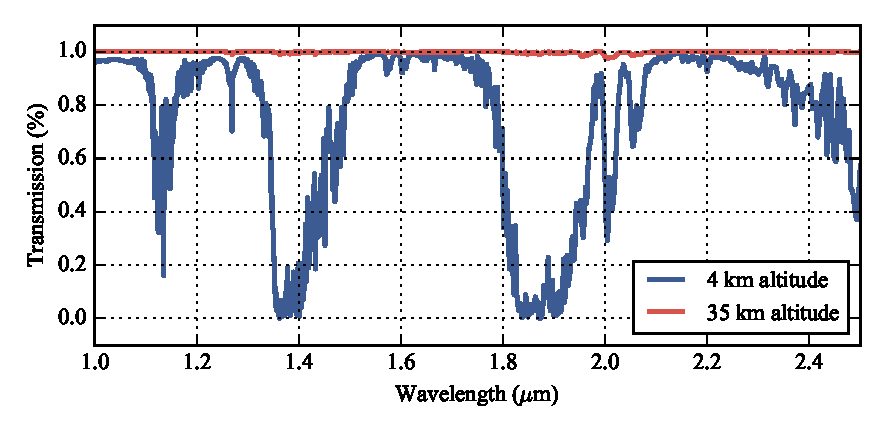
\includegraphics[width=\textwidth]{Figures/BETTII_atmo_transmission.pdf}
\caption{Model atmospheric transmission, from \cite{Rizzo:2012jp}}
\label{fig:trans}
\end{center}
\end{figure}


\subsection{Targets}


\subsubsection{Calibrators}
\subsubsection{Science targets}
introduce the SOFIA work here

